\documentclass[conference]{IEEEtran}

\usepackage{cite}
\usepackage{amsmath,amssymb,amsfonts}
\usepackage{amsthm}
\usepackage[table]{xcolor}
\definecolor{RWStripe}{gray}{0.95}
\definecolor{RWThis}{gray}{0.90}
\usepackage{array,multirow,makecell}
\usepackage{booktabs}
\usepackage{float}
\usepackage{graphicx}
\usepackage{mathrsfs}
\usepackage{mdwmath}
% \usepackage{mdwtab} % Disabled because it overrides colortbl row shading; no mdwtab-specific commands are used.
\usepackage{tabularx}
\usepackage{textcomp}
\usepackage[hyphens]{url}
\Urlmuskip=0mu plus 1mu\relax
% \usepackage{xcolor}
\usepackage{xspace}
\usepackage[english]{babel}
\usepackage{algorithm}
\usepackage{algpseudocode}
\usepackage{acronym}
% Acronym definitions in the preamble use \acrodef.
\acrodef{fl}[FL]{Federated Learning}
\acrodef{cl}[CL]{Collaborative Learning}
\acrodef{dp}[DP]{Differential Privacy}
\acrodef{nn}[NN]{Neural Network}
\acrodef{nids}[NIDS]{Network Intrusion Detection System}

\pagestyle{plain}

\newcommand{\red}[1]{{\color{red}{#1}}}
\newcommand{\add}[1]{{\color{red}{#1}}}
\newcolumntype{P}[1]{>{\centering\arraybackslash}p{#1}}
\newcolumntype{M}[1]{>{\centering\arraybackslash}m{#1}}
\newcolumntype{L}[1]{>{\raggedright\arraybackslash}p{#1}}
\newcolumntype{Y}{>{\raggedright\arraybackslash}X}
\theoremstyle{definition}
\newtheorem{definition}{Definition}[section]
\newtheorem{theorem}{Theorem}[section]
\newtheorem{proposition}[theorem]{Proposition}
\newtheorem{corollary}[theorem]{Corollary}
\newcommand{\cf}{\hbox{{cf.}}\xspace}
\newcommand{\etal}{\hbox{{et al.}}\xspace}
\newcommand{\eg}{\hbox{{e.g.}}\xspace}
\newcommand{\ie}{\hbox{{i.e.}}\xspace}
\newcommand{\wrt}{\hbox{{w.r.t.}}\xspace}
\newcommand{\etc}{\hbox{{etc.}}\xspace}
\newcommand{\perse}{\hbox{{per se.}}\xspace}
\newcommand{\aka}{\hbox{{a.k.a.}}\xspace}
\newcommand{\Fname}{\textsc{SiloStitch}\xspace}
\newcommand{\bheading}[1]{\noindent\textbf{#1.}\xspace}
\newcommand{\dt}[1]{\textbf{\textcolor{blue}{[Tian: #1]}}}
\newcommand{\fullmark}{\ensuremath{\checkmark}}
\newcommand{\partialmark}{\ensuremath{\bullet}}
\newcommand{\emptymark}{\ensuremath{\circ}}
\newcommand{\namark}{\ensuremath{\text{--}}}

\hyphenation{op-tical net-works semi-conduc-tor}

\newenvironment{packeditemize}{
\begin{list}{$\bullet$}{
\setlength{\labelwidth}{8pt}
\setlength{\itemsep}{0pt}
\setlength{\leftmargin}{\labelwidth}
\addtolength{\leftmargin}{\labelsep}
\setlength{\parindent}{0pt}
\setlength{\listparindent}{\parindent}
\setlength{\parsep}{0pt}
\setlength{\topsep}{3pt}}}{\end{list}}

\begin{document}

\title{\red{\Fname: Integrating Pretrained Intrusion Detectors under Deployment Budgets}}

% Anonymous submission: author names, affiliations, and email addresses are omitted.
\author{}

\maketitle

\begin{abstract}
\red{Organizations may retain intrusion detectors after the records used to
train them become unavailable. However, deploying the entire retained pool
can exceed a resource budget. Selecting detectors only by average current
utility can discard the sole feasible detector that supports an important
class, while historical support alone says little about current competence.
We present \Fname, which integrates pretrained detectors under a hard budget
without changing them. The method aligns their probability outputs and uses
held-out records to form a calibration-eligible pool. It then computes the
maximum weighted source-class support exactly and compares current prediction
behavior only among sets that preserve this value. Using a disjoint fit
partition, the coordinator trains one shared stacker over the selected
probability blocks. Clients may add Laplace noise to these blocks before
upload. We establish simultaneous post-selection calibration, exact primary
optimization with an explicit capacity guard, and a local certificate for
secondary refinement. We also prove label-conditional local privacy for score
uploads and characterize when current class-conditional utility supports
historical class claims under bounded client-mixture change. Across four
cybersecurity datasets, a 50\% target budget reduces logical payload by
49.3--50.4\%. Macro-F1 remains within 0.0052 of all encoders on three datasets;
DDOS exhibits a 0.0258 gap.}
\end{abstract}

\IEEEpeerreviewmaketitle

\section{Introduction}
\label{sec:introduction}

\red{Operational networks often keep intrusion detectors longer than the
records used to train them. Storage and retention policies may remove
historical traffic logs~\cite{acsc2024logging,microsoft2026retention}, even as
traffic and attack patterns continue to change~\cite{nist2023airmf}.
Detectors trained in different organizations may therefore preserve different
class support and prediction behavior. Retraining them through another
collaborative process would require suitable source data and permission to
update the contributed models~\cite{federated_learning,Fedprox,ditto2021}.
We study post-training integration instead: clients contribute pretrained
detectors, and the collaboration leaves their parameters unchanged.}

\red{A deployment may still be unable to use every contributed detector.
Distributing a model and processing its aligned probability block both consume
resources, so the collaboration must select a subset under a hard budget. A
utility-only rule may spend that budget on several detectors that repeat
common behavior while omitting the sole feasible detector whose source data
support a less frequent or high-priority class. Source support alone has the
opposite weakness: it can preserve nominal breadth while retaining detectors
that perform poorly or add little beyond those already chosen.}

\red{One might combine support and current utility in a weighted sum. Yet any
fixed coefficient allows enough secondary gain to compensate for a positive
support loss when the instance contains a sufficiently small coverage gap.
The two quantities therefore play different roles. Source-side class support
states what the deployment should retain whenever the budget permits, whereas
current behavior distinguishes sets only after that requirement has been met.
\Fname represents this priority as two ordered decisions rather than another
scale-dependent tradeoff.}

\red{To compare heterogeneous candidates, \Fname translates every native
probability vector into a shared target-class order and reserves one output
for unsupported labels. Held-out labeled records then provide normalized
Brier utilities, class-conditional lower utilities, and prediction
signatures. Separately, fixed source-support counts describe which classes a
detector encountered during training, while a logical-byte cost represents
model distribution and the probability block used by the shared stacker.
These quantities allow the method to distinguish historical support, current
behavior, and deployment cost without treating them as interchangeable.}

\red{The selector first removes candidates that fail the calibration gate.
Within the remaining pool, a sparse bitmask dynamic program obtains the
largest weighted source-class support available under the budget. Only sets
with that value enter the secondary comparison, which rewards record utility,
conservative class utility, and representative prediction behavior. A local
fill-and-swap procedure uses any remaining budget without lowering the primary
value. Thus, \Fname combines exact primary optimization with a
coverage-preserving fill-and-swap refinement.}

\red{Once selection ends, the coordinator trains one shared stacker on a
disjoint fit partition using the selected aligned probability
blocks~\cite{wolpert1992stacked}. Separate partitions for candidate fitting,
selection calibration, stacker fitting, and sealed testing prevent test labels
from influencing selection or training. When local score protection is
enabled, each client perturbs every selected probability block with Laplace
noise before upload. This release provides label-conditional local privacy for
feature-derived scores under the label-fixed neighboring relation used in our
analysis.}

\red{Our analysis follows these dependencies. A simultaneous calibration
event keeps detector-level and class-conditional bounds valid after adaptive
selection. We then show that the primary problem is NP-hard but solved exactly
by the implemented bitmask program within its registered state cap. The
secondary objective is monotone and submodular, and the production refinement
provides a coverage-preserving one-swap certificate. The Laplace analysis
proves local privacy for one uploaded score block and accounts for composition
across selected blocks. Finally, an
effective-coverage certificate identifies when current class-conditional
utility supports historical class claims, including under bounded changes in
the client mixture.}

\red{Our evaluation uses four cybersecurity datasets with 66 candidate
detectors per task. At a 50\% target budget, \Fname reduces logical payload by
49.3--50.4\%; its Macro-F1 remains within 0.0052 of all encoders on MALDROID,
DARKNET, and DOH, while DDOS shows a 0.0258 gap. The primary solver matches
exhaustive search throughout the oracle suite, and a seven-level Laplace
profile quantifies the utility response to score perturbation.}

\red{Together, these choices lead to three contributions.}
\begin{packeditemize}
    \item \red{First, we formulate budgeted post-training detector integration as an ordered decision that separates source-side class support from current predictive evidence.}
    \item \red{Second, we design \Fname to align frozen detectors, maximize weighted support exactly, refine current behavior without sacrificing that support, and fit one shared stacker from optionally perturbed scores.}
    \item \red{Finally, we establish post-selection calibration, characterize the exact and local parts of the solver, prove label-conditional privacy for score uploads, and analyze effective coverage under client-mixture change.}
\end{packeditemize}




\section{Background and Related Work}
\label{sec:related}
\red{This section distinguishes post-training detector integration from
collaborative retraining, reviews nearby integration and selection methods,
and introduces the privacy notion used for score uploads.}
\subsection{\red{Training-Time Collaborative Detection}}

\red{In conventional federated learning, clients retain local data while jointly building or updating a base model~\cite{federated_learning,Fedprox,ditto2021}. Recent NIDS systems follow this training-time pattern across detector designs~\cite{pourahmadi2023fedoe,mao2025fedinnid}. For example, Entente jointly trains graph-based detectors from distributed network logs~\cite{xu2026entente}. Federated tree methods likewise build their base models during collaboration~\cite{federboost,dpfedtree_ccs22}. Thus, these methods require local data while training the base detector. We instead freeze every detector before collaboration and learn only a personalized composer over its outputs.}

\red{Existing methods also adapt network-traffic classifier or detector training to specific deployment problems, such as noisy labels or network shift~\cite{qing2024rapier,xie2023rosetta,yang2026cold}. For example, CoLD filters noisy labels before training a detector~\cite{yang2026cold}. These methods modify the detector itself. We instead keep every detector frozen and learn a composer from limited current site data.}

\subsection{\red{Frozen Model Reuse and Personalization}}

\red{Some methods reuse pretrained models when their original training data are unavailable. For example, Old Dogs learns one target classifier from pretrained source networks without using source data~\cite{old_dogs2019}. In a multiparty setting, HMR exchanges selected examples and calibrates the reused models during collaboration~\cite{wu2019hmr}. Likewise, Ma et al. keep local models frozen but send per-example representations of aligned samples to a central server~\cite{ma2023consensus}. We instead keep all detectors frozen, keep per-example outputs local, and make adoption site-specific.}

\red{Other methods first train local classifiers from current data and then learn a second-stage model. F-BIDS and Fed-MStacking follow this pattern~\cite{aouedi2023fbids,qiu2024fedmstacking}. Meanwhile, personalized federated learning updates base models during collaboration~\cite{fedfomo2021,ditto2021}. We instead start from detectors frozen before collaboration and train only the composer.}

\subsection{\red{Protected Collaboration and Local Adoption}}

\red{The two stages raise different questions. During candidate construction, keeping current site data local does not protect the composer gradient sent by each site. We therefore use secure aggregation so that the coordinator receives only the aggregate gradient and no individual gradient in plaintext when sites do not collude with it~\cite{bonawitz2017secureaggregation}. By comparison, FedDef perturbs training inputs to reduce gradient-reconstruction leakage in federated NIDSs~\cite{chen2023feddef}. Moreover, differential privacy limits how much the output distribution can change between neighboring datasets~\cite{dwork2006calibrating}. However, our protocol provides neither differential privacy nor protection against inference from the aggregates.}

\red{Deployment authorization begins only after construction ends. When old training data are unavailable or do not match the target distribution, Active Comparison uses new labels to compare a fixed baseline and challenger~\cite{sawade2012activecomparison}. Separately, Learn Then Test evaluates prespecified risk hypotheses on independent calibration data~\cite{angelopoulos2025ltt}. We likewise freeze the candidate before using audit data, but couple this decision to the preceding example-local construction stage and bound excess risk relative to each site's audited incumbent. Existing protection and comparison mechanisms therefore address the two stages separately rather than the complete post-training deployment contract.}

\section{\red{Problem Statement}}
\label{sec:problem}

\subsection{\red{System Setting}}

\red{We formalize post-training federation. We distinguish package owners from deployment sites, although one organization may have both roles. Before collaboration, each owner freezes a detector and registers it. A trusted registry distributes the same versioned package pool to every site. The registry checks that each package matches the registered version, but it does not certify its behavior. During collaboration, the sites run the packages locally, while a separate coordinator trains a shared composer from secure aggregates.}

\red{More formally, we consider $J\ge2$ deployment sites that reuse $m$ intrusion detectors. Every package follows the same input and class-score interface over $C$ classes. For detector $i$, we write its frozen package and valid score output as}
\begin{equation}
\red{\mathcal M_i=(T_i,f_i), \qquad q_i(x)=f_i(T_i(x))\in\Delta^{C-1},}
\label{eq:frozen_package}
\end{equation}
\red{where $T_i$ and $f_i$ form the fixed inference pipeline, and $q_i$ is its normalized class-score output. We keep $T_i$ and $f_i$ fixed.}

\red{To identify the package deployed at each site, we use the map $\iota:\{1,\ldots,J\}\rightarrow\{1,\ldots,m\}$. At site $D_j$, the deployed package produces}
\begin{equation}
\red{b_j(x)=q_{\iota(j)}(x)}
\label{eq:incumbent}
\end{equation}
\red{and we call $b_j$ the raw incumbent output. A site may deploy a package from another organization, so we do not require $m=J$. The audit later compares its candidate with a fixed transformation of $b_j$. We call this comparator the audited incumbent and define it in Section~\ref{sec:approach}.}

\red{We call the labeled local observations obtained from the package pool \emph{current site data}. For fitting and audit, each site divides these data into a nonempty fit set $B_j^{fit}$ and a held-out audit set $B_j^{safe}$. We use $B_j^{fit}$ for shared training and local personalization, and we also use it to fix every audit choice. We reserve $B_j^{safe}$ for the final adoption audit. We do not assume that the current site distribution matches the unknown training distribution of any package.}

\red{During shared training, each site keeps its per-example current site data local and submits its composer gradient through secure aggregation. Local personalization and the adoption audit send no message to the coordinator.}

\subsection{\red{Problem Formulation}}

\red{Given the frozen package pool and current site data, each site needs both a candidate and an authorization decision. Candidate construction uses only the fit sets and seeks to reduce site-level fit loss by sharing correction structure when it is useful. Authorization is a separate constraint: site $j$ preselects a nonempty set of audit metrics $\mathcal E_j$ and a tolerance $\eta_{j,e}$ for every $e\in\mathcal E_j$, then deploys the frozen candidate only when a valid local audit places an upper bound on its excess risk over the audited incumbent within every tolerance. Thus, construction searches for utility without access to the audit set, while authorization determines whether that candidate may replace the incumbent.}

\subsection{\red{Threat Model}}
\label{sec:threat_model}

\red{We consider an honest-but-curious coordinator as the privacy adversary. It follows the prescribed protocol but may analyze its training view across rounds. In each completed round, this view includes the decoded aggregate gradient and the resulting shared composer. The coordinator receives no message from local personalization or the adoption audit.}

\red{We assume that the deployment sites follow the protocol and that none colludes with the coordinator. We also assume the standard authenticated communication required by secure aggregation. We trust the registry only to distribute the same registered pool to every site. Each site verifies this pool and runs its packages unchanged. We make no accuracy assumption about a package, but we model it as a fixed inference function. Executable code that violates this model is outside our scope.}

\red{For adoption, we assume that the held-out labels are correct for the audited task and fixed independently of the candidate. A systematic labeling error changes the risk controlled by our result.}

\red{Under these assumptions, per-example current site data remain local, and the coordinator does not receive any site's encoded composer gradient in plaintext. However, the shared composer may still leak information, and we provide no differential privacy. We do not protect against inference by another site or against active protocol deviations. Finally, because deployment sites execute the packages locally, we do not hide the packages from them.}


\section{\red{Design of \Fname}}
\label{sec:approach}

\begin{figure*}[htbp]
    \centering
    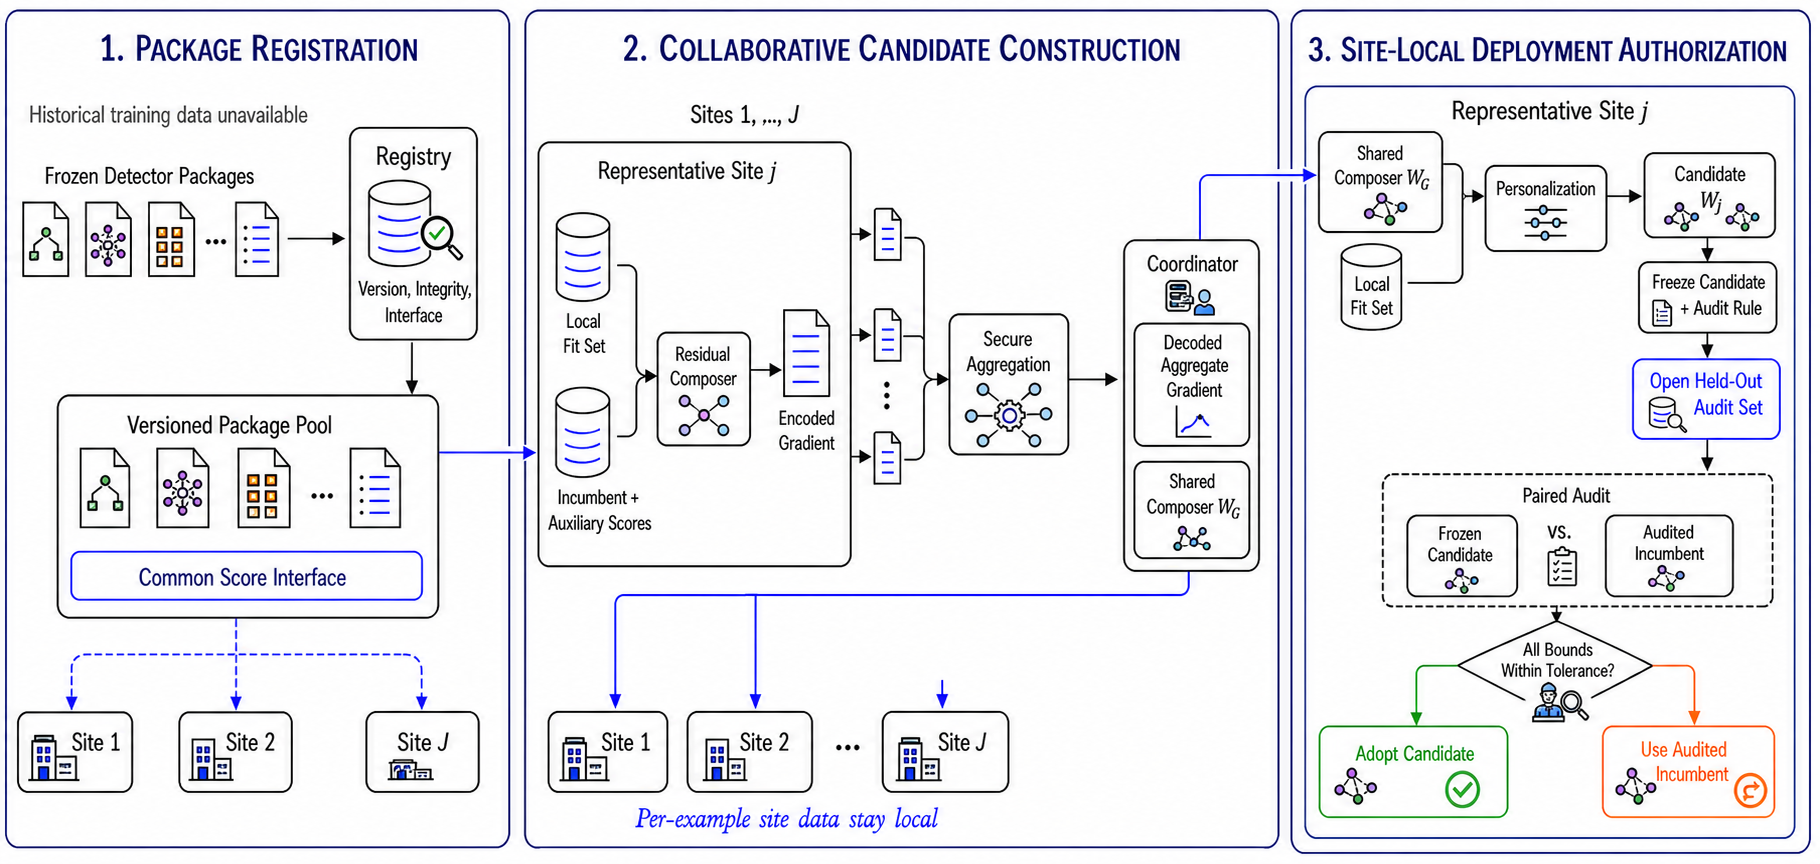
\includegraphics[width=\linewidth]{figures/post-training-federation-overview-v4.png}
    \caption{\red{Overview of \Fname through deployment authorization. Each site learns a personalized composer and audits it before deployment. The coordinator receives aggregated composer gradients, while each site keeps per-example scores and its personalized composer local. Section~\ref{sec:approach} describes the separate runtime response after authorization.}}
    \label{fig:workflow}
\end{figure*}

\subsection{\red{Overview}}

\red{Even without its historical training material, an auxiliary detector may help correct incumbent errors on current site data. We therefore compose only final scores and learn corrections relative to the incumbent. This design gives the sites a common correction space and retains an exact no-change state. When correction structure is shared, federated training can pool signals across sites and provide a common prior. However, package utility may differ by site, so the shared composer remains a starting point for local personalization. The resulting predictor remains a candidate until a held-out audit authorizes its deployment. Candidate construction and deployment authorization are therefore separate by design: collaboration can change the candidate, but only the local audit can change deployment.}

\red{As shown in Figure~\ref{fig:workflow}, the workflow begins with package registration. Before fitting, every site verifies the complete pool manifest. If any site finds a mismatch, the collaboration stops and the sites keep their existing deployments. Each site then builds incumbent-anchored inputs from $B_j^{fit}$ and trains the shared composer from securely aggregated, encoded gradients. After the coordinator returns $W_G$, each site personalizes the composer and freezes its candidate. Only then does the site open $B_j^{safe}$ and decide whether to adopt the candidate.}

\subsection{\red{Incumbent-Anchored Composer}}

\red{Let $W$ denote the composer weights. We design the composer so that $W=0$ reproduces the incumbent after the same smoothing used for every package. We therefore express each auxiliary score relative to the incumbent. To avoid $\log 0$, we first smooth each score vector. For $0<\lambda_0<1$, define}
\begin{equation}
\red{\mathcal S_{\lambda_0}(p)=(1-\lambda_0)p+\frac{\lambda_0}{C}\mathbf 1,}
\label{eq:smoothing_base}
\end{equation}
\red{and let $\widetilde q_i=\mathcal S_{\lambda_0}(q_i)$ and $\widetilde b_j=\mathcal S_{\lambda_0}(b_j)$. The protocol fixes $\lambda_0$ before any site uses current data.}

\red{Let $v_{ij}(x)\in\{0,1\}$ indicate whether detector $i$ returns a valid score for $x$ at site $j$. The common interface defines a no-score state for auxiliary packages, which this mask records throughout the workflow. The incumbent must always return a valid score, so the zero branch below applies only to auxiliary packages. We define}
\begin{equation}
\red{
r_{ij}(x)=
\begin{cases}
\log \widetilde q_i(x)-\log \widetilde b_j(x), & v_{ij}(x)=1,\\
\mathbf 0, & v_{ij}(x)=0.
\end{cases}}
\label{eq:score_residual}
\end{equation}
\red{We reserve a fixed feature block for every registered package. We then form}
\begin{equation}
\red{
\phi_j(x)=
\left[
1,\{v_{ij}(x)\}_{i=1}^{m},
\log \widetilde b_j(x)^{\mathsf T},
\{r_{ij}(x)^{\mathsf T}\}_{i=1}^{m}
\right]^{\mathsf T}.}
\label{eq:composer_feature}
\end{equation}

\red{We use a linear residual head:}
\begin{equation}
\red{
h_{j,W}(x)=
\operatorname{softmax}\!\left(
\log \widetilde b_j(x)+W\phi_j(x)
\right),}
\label{eq:residual_head}
\end{equation}
\red{where $W\in\mathbb R^{C\times(1+m+C+mC)}$. When $W=0$, $h_{j,0}(x)=\widetilde b_j(x)$. Thus, the residual head starts from the smoothed incumbent and fits corrections using current site data.}

\red{Before shared training begins, every site checks that its incumbent is valid throughout $B_j^{fit}$. If any check fails, the collaboration stops and produces no candidate.}

\subsection{\red{Federated Composer Training}}

\red{We train the composer with the negative log-likelihood of Eq.~\ref{eq:residual_head}. For site $j$, the local fit loss is}
\begin{equation}
\red{
\widehat R_j^{fit}(W)=
\frac{1}{|B_j^{fit}|}
\sum_{(x,y)\in B_j^{fit}}
-\log h_{j,W}(x)_y.}
\label{eq:fit_risk}
\end{equation}
\red{We give every site equal weight. For a public radius $R>0$ fixed before any site uses current data, we minimize}
\begin{equation}
\red{
\min_{\lVert W\rVert_F\le R}
\frac{1}{J}\sum_{j=1}^{J}\widehat R_j^{fit}(W).}
\label{eq:global_objective}
\end{equation}

\red{Because $\phi_j(x)$ and $\widetilde b_j(x)$ are fixed, the negative log-likelihood is convex in $W$. Thus, Eq.~\ref{eq:global_objective} is a convex problem.}

\red{We initialize $W^{(0)}=0$ and fix the optimization schedule before any site uses current data. At round $t$, site $j$ computes the full-batch gradient $g_j^{(t)}=\nabla\widehat R_j^{fit}(W^{(t)})$. Secure aggregation gives the coordinator only their sum. It averages this sum and takes one projected step. When training completes, the final iterate becomes the shared composer $W_G$.}

\red{We use a fixed-point encoding for secure aggregation~\cite{bonawitz2017secureaggregation}. Before training, we fix a public coordinate bound $G$, a scale $s$, and a modulus $Q>2J\lceil sG\rceil$. Each site clips and encodes its gradient under these parameters, which prevent the aggregate from wrapping around. This encoding changes the optimization only through the fixed clipping and quantization.}

\red{We require the fixed set of $J$ sites in every completed round. A dropout aborts the round. If repeated dropout prevents training from completing, no candidate is produced and every site keeps its existing deployment. Section~\ref{sec:threat_model} states the separate privacy boundary.}

\subsection{\red{Local Personalization}}

\red{Because current traffic may differ across sites, we adapt $W_G$ rather than deploy it directly. Site $j$ selects $\mu_j>0$ with its fit data and solves}
\begin{equation}
\red{
W_j=
\arg\min_{\lVert W\rVert_F\le R}
\widehat R_j^{fit}(W)
+\mu_j\lVert W-W_G\rVert_F^2,}
\label{eq:local_objective}
\end{equation}
\red{We keep $W_j$ at site $j$. Because the fit loss is convex, the local objective is strongly convex when $\mu_j>0$. Here, $\mu_j$ balances the shared composer against local fitting, while $W_G$ remains an anchor rather than a common final detector.}

\red{Because $W_G$ is feasible in Eq.~\ref{eq:local_objective}, optimality gives}
\begin{equation}
\red{\widehat R_j^{fit}(W_j)
+\mu_j\lVert W_j-W_G\rVert_F^2
\le \widehat R_j^{fit}(W_G).}
\label{eq:personalization_dominance}
\end{equation}
\red{Thus, exact local personalization does not increase fit loss relative to the shared composer. This fit-side property does not justify deployment on the audit distribution.}

\subsection{\red{Deployment Audit}}

\red{Local fitting produces a candidate but does not justify deployment. Before opening $B_j^{safe}$, we therefore fix $W_j$, the complete audit configuration, and a value $0<\lambda_a<1$. We use $\lambda_a$ only to bound probability-based audit losses; the transformation preserves the predicted class. We then define the audited pair as follows:}
\begin{equation}
\red{
\overline h_j=\mathcal S_{\lambda_a}(h_{j,W_j}),
\qquad
\overline b_j=\mathcal S_{\lambda_a}(\widetilde b_j),}
\label{eq:audit_wrapper}
\end{equation}
\red{Here, $\overline h_j$ is the frozen candidate and $\overline b_j$ is the audited incumbent. A valid audit compares and deploys only these two predictors. Thus, the audited incumbent is not the raw probability output $b_j$.}

\red{After opening $B_j^{safe}$, we construct the configured audit blocks and compare $\overline h_j$ with $\overline b_j$. For every preselected metric, a valid audit must produce the precommitted number $n_{j,e}\ge2$ of complete blocks. If any comparison cannot be completed as fixed, the audit is invalid. Section~\ref{sec:adoption_analysis} states the sampling assumption and defines the upper bound $U_{j,e}$. For a valid audit, the site adopts the candidate only when $U_{j,e}\le\eta_{j,e}$ for every preselected metric. Otherwise, it uses $\overline b_j$.}

\red{The mask covers only the interface-defined no-score state. Any other package failure during the audit, including an incumbent failure, makes the audit invalid, so the site keeps its existing deployment.}

\red{After deployment, the audited incumbent provides the runtime fallback. If an adopted candidate no longer executes as audited, the site uses $\overline b_j$; if $\overline b_j$ is unavailable, it abstains and alerts the operator. An interface change requires a new candidate and another audit.}


\section{\red{Adoption Analysis}}
\label{sec:adoption_analysis}

\red{Candidate construction and deployment authorization are deliberately decoupled. Once a candidate and its audit rule are frozen, the analysis depends on the paired audit distribution rather than on the fitting algorithm. We first show that unlabeled outputs alone cannot generally identify the predictor with lower current classification error. We then establish a simultaneous adoption guarantee and characterize when the candidate's population excess risk lies below the adoption threshold by a positive margin.}

\subsection{\red{Limits of Unlabeled Adoption}}

\red{We first ask whether a site can decide adoption without current labels. Fix one site, and let $\widehat h$ and $\widehat b$ be the hard predictions of its frozen candidate and audited incumbent. Let $O$ denote any label-free view generated from the input distribution and these two fixed predictors. We allow fixed side information as long as it imposes no restriction on $P(Y\mid X)$.}

\begin{proposition}[\red{Unlabeled relative risk is not identifiable}]
\label{prop:unlabeled_limit}
\red{Fix a marginal distribution $P_X$, and suppose}
\begin{equation}
\red{\rho=\Pr_{P_X}[\widehat h(X)\ne\widehat b(X)]>0.}
\label{eq:disagreement_mass}
\end{equation}
\red{For any possibly randomized rule $\mathcal A(O)\in\{\mathsf{adopt},\mathsf{retain}\}$ based on any number of unlabeled observations, and any $0<\gamma\le\rho$, there are two joint distributions $P_+$ and $P_-$ over $(X,Y)$ that induce the same distribution of $O$ but satisfy}
\begin{equation}
\red{\Delta_{01}(P_+)=-\gamma,
\qquad
\Delta_{01}(P_-)=\gamma,}
\label{eq:two_world_risks}
\end{equation}
\red{where $\Delta_{01}(P)=R_{01,P}(\widehat h)-R_{01,P}(\widehat b)$. Moreover,}
\begin{equation}
\red{\Pr_{P_+}[\mathcal A=\mathsf{retain}]
+\Pr_{P_-}[\mathcal A=\mathsf{adopt}]=1.}
\label{eq:unlabeled_error_sum}
\end{equation}
\red{Consequently, one of these two error probabilities is at least $1/2$.}
\end{proposition}

\begin{proof}
\red{Let $S=\{x:\widehat h(x)\ne\widehat b(x)\}$ and $a=\gamma/\rho$. Both worlds draw $X$ from $P_X$. Outside $S$, they set $Y$ to the common prediction. On $S$, $P_+$ sets $Y=\widehat h(X)$ with probability $(1+a)/2$ and $Y=\widehat b(X)$ otherwise; $P_-$ exchanges these probabilities. Thus, the worlds expose the same unlabeled observations but have relative risks $-\gamma$ and $\gamma$. The rule adopts with the same probability, say $q$, in both worlds, so its two error probabilities are $1-q$ and $q$.}
\end{proof}

\red{Proposition~\ref{prop:unlabeled_limit} does not rule out unlabeled adoption under an additional assumption that links labels to the observed information. It also permits a site to retain its incumbent. Instead, it shows that unlabeled observations alone cannot generally identify even which fixed predictor has lower classification error. We therefore use current labels for the adoption audit.}

\subsection{\red{Simultaneous Incumbent-Relative Adoption}}

\red{Let $\mathcal T$ denote all protocol choices and outputs fixed before any audit set is opened. In particular, $\mathcal T$ fixes both predictors, the complete audit configuration, and every block count $n_{j,e}$. We condition on $\mathcal T$.}

\red{For each site--metric pair, the fixed rule draws $n_{j,e}$ blocks $\mathcal B_{j,e,1},\ldots,\mathcal B_{j,e,n_{j,e}}$ from $B_j^{safe}$. Given $\mathcal T$, we assume that these blocks are independent and identically distributed. For a class-conditional metric, the rule draws fixed-size blocks from the corresponding class. We allow dependence among flows in the same block. We also allow metrics to reuse records, so the proof does not assume independence across metrics.}

\red{For the bounded loss $\ell_e$ of audit metric $e$, define}
\begin{equation}
\red{
\begin{aligned}
L_{j,e}(g;\mathcal B)
&=\frac{1}{|\mathcal B|}
\sum_{(x,y)\in\mathcal B}\ell_e(g(x),y),\\
R_{j,e}(g)&=\mathbb E[L_{j,e}(g;\mathcal B)\mid\mathcal T].
\end{aligned}}
\label{eq:block_risk}
\end{equation}
\red{We compare the candidate and audited incumbent on each block:}
\begin{equation}
\red{
\begin{aligned}
D_{j,e,r}
&=L_{j,e}(\overline h_j;\mathcal B_{j,e,r})
-L_{j,e}(\overline b_j;\mathcal B_{j,e,r}),\\
\Delta_{j,e}&=R_{j,e}(\overline h_j)-R_{j,e}(\overline b_j).
\end{aligned}}
\label{eq:paired_difference}
\end{equation}
\red{For a classification-error audit, pairing has a direct variance interpretation. The per-record loss difference is zero whenever the two hard predictions agree. Jensen's inequality therefore gives}
\begin{equation}
\red{\operatorname{Var}(D_{j,e,r}\mid\mathcal T)
\le \mathbb E[D_{j,e,r}^2\mid\mathcal T]
\le \rho_{j,e},}
\label{eq:disagreement_variance}
\end{equation}
\red{where $\rho_{j,e}$ is the expected fraction of records in an audit block on which the two predictions disagree. Hence, incumbent-relative comparison can be sharper when the candidate changes few predictions, although the anchor alone does not guarantee small disagreement.}
\red{Assume $D_{j,e,r}\in[-M_{j,e},M_{j,e}]$. Let}
\begin{equation}
\red{
\begin{aligned}
\overline D_{j,e}&=\frac{1}{n_{j,e}}\sum_{r=1}^{n_{j,e}}D_{j,e,r},\\
\widehat V_{j,e}&=
\frac{1}{n_{j,e}-1}
\sum_{r=1}^{n_{j,e}}(D_{j,e,r}-\overline D_{j,e})^2.
\end{aligned}}
\label{eq:paired_variance}
\end{equation}
\red{For a per-pair failure probability $\alpha_{j,e}\in(0,1)$, we apply the empirical Bernstein bound~\cite{maurer2009empiricalbernstein} to obtain}
\begin{equation}
\red{
U_{j,e}=\overline D_{j,e}
+\sqrt{\frac{2\widehat V_{j,e}\log(2/\alpha_{j,e})}{n_{j,e}}}
+\frac{14M_{j,e}\log(2/\alpha_{j,e})}{3(n_{j,e}-1)}.}
\label{eq:bernstein_ucb}
\end{equation}

\red{Thus, $U_{j,e}$ is an upper confidence bound on the candidate's excess risk for one site and audit metric. We next obtain a simultaneous bound over all site--metric pairs.}

\begin{theorem}[\red{Simultaneous adoption relative to the audited incumbent}]
\red{Before the audit, fix $\{\mathcal E_j\}_{j=1}^{J}$, the values $\alpha_{j,e}\in(0,1)$ and $\eta_{j,e}\ge0$ for every $e\in\mathcal E_j$, and $\alpha_{\mathrm{tot}}\in(0,1)$. Suppose that $n_{j,e}\ge2$, the variables $D_{j,e,1},\ldots,D_{j,e,n_{j,e}}$ are i.i.d. in $[-M_{j,e},M_{j,e}]$ given $\mathcal T$, and}
\begin{equation}
\red{\sum_{j=1}^{J}\sum_{e\in\mathcal E_j}\alpha_{j,e}
\le\alpha_{\mathrm{tot}}.}
\label{eq:failure_budget}
\end{equation}
\red{Then, conditional on $\mathcal T$, with probability at least $1-\alpha_{\mathrm{tot}}$, $\Delta_{j,e}\le U_{j,e}$ holds for every site and audit metric. Let site $j$ deploy $\overline h_j$ only when $U_{j,e}\le\eta_{j,e}$ for every $e\in\mathcal E_j$ and otherwise deploy $\overline b_j$. Under the same event,}
\begin{equation}
\red{
R_{j,e}(h_j^{\mathrm{deploy}})-R_{j,e}(\overline b_j)
\le\eta_{j,e},
\qquad e\in\mathcal E_j.}
\label{eq:joint_adoption}
\end{equation}
\end{theorem}

\begin{proof}
\red{For one site and audit metric, the empirical Bernstein inequality applied to $D_{j,e,r}$ gives $\Pr(\Delta_{j,e}>U_{j,e}\mid\mathcal T)\le\alpha_{j,e}$. Next, a union bound and Eq.~\ref{eq:failure_budget} give the simultaneous result. If every audit metric passes, Eq.~\ref{eq:joint_adoption} follows from $\Delta_{j,e}\le U_{j,e}\le\eta_{j,e}$. Otherwise, $h_j^{\mathrm{deploy}}=\overline b_j$, and the risk difference is zero.}
\end{proof}

\begin{corollary}[\red{Power of the local audit}]
\label{cor:audit_power}
\red{Condition on $\mathcal T$ and fix one site--metric pair. Suppose that $n\ge2$, the paired differences $D_1,\ldots,D_n$ are i.i.d. in $[-M,M]$, and $\alpha,\beta\in(0,1)$. If the population excess risk satisfies $\Delta\le\eta-\gamma$ for some $\gamma>0$, and}
\begin{equation}
\red{
M\sqrt{\frac{2\log(1/\beta)}{n}}
+M\sqrt{\frac{2\log(2/\alpha)}{n-1}}
+\frac{14M\log(2/\alpha)}{3(n-1)}
\le\gamma,}
\label{eq:audit_power_condition}
\end{equation}
\red{then $\Pr(U\le\eta\mid\mathcal T)\ge1-\beta$. If the condition holds for every metric $e$ at site $j$ and $\sum_{e\in\mathcal E_j}\beta_{j,e}\le\beta_j$, then site $j$ accepts the candidate with conditional probability at least $1-\beta_j$.}
\end{corollary}

\begin{proof}
\red{Because $D_r\in[-M,M]$, the sample variance satisfies $\widehat V\le nM^2/(n-1)$. Hoeffding's inequality gives $\overline D\le\Delta+M\sqrt{2\log(1/\beta)/n}$ with probability at least $1-\beta$. Substituting these two bounds into Eq.~\ref{eq:bernstein_ucb} and using Eq.~\ref{eq:audit_power_condition} gives $U\le\eta$. A union bound gives the statement for all metrics; no independence across metrics is needed.}
\end{proof}

\red{A sufficient audit size in Corollary~\ref{cor:audit_power} scales as}
\begin{equation}
\red{n=O\!\left(1+
\frac{M^2}{\gamma^2}
\left[\log\frac{2}{\alpha}+\log\frac{1}{\beta}\right]
+\frac{M}{\gamma}\log\frac{2}{\alpha}
\right)}
\label{eq:audit_power_rate}
\end{equation}
\red{independent blocks. This sufficient condition is conservative because it upper-bounds the sample variance, whereas the actual audit uses the observed paired variance.}

\red{For negative log-likelihood, Eq.~\ref{eq:audit_wrapper} makes every class probability at least $\lambda_a/C$. Thus, we set $M_{j,e}=\log(C/\lambda_a)$. For a conditional error rate, we instead use its corresponding class-conditional blocks and set $M_{j,e}=1$. For example, FPR uses benign blocks.}

\subsection{\red{Scope of the Guarantee}}

\red{Because we condition on the complete pre-audit state, the guarantee treats the candidate and audit rule as fixed. It therefore requires neither exact optimizer convergence nor an accuracy assumption about a package. Here, $n_{j,e}$ counts independent labeled blocks rather than individual flows. More blocks and lower paired variance tighten Eq.~\ref{eq:bernstein_ucb}, while a power guarantee also requires a positive margin below the adoption threshold.}

\red{The guarantee applies to one frozen candidate and the fixed audit-block distribution. In particular, non-overlapping windows alone do not establish the block assumption. After a post-audit shift, the prior guarantee no longer applies, and a new adoption claim requires another audit.}

\red{The guarantee also applies only to the preselected metrics. For example, NLL control does not imply Macro-F1 control. Moreover, we compare the candidate with the audited incumbent and do not show that the incumbent itself is safe. We assume that both audited predictors execute as fixed; post-audit package failures and the resulting fallback policy are outside this statistical guarantee.}

\begingroup
\color{red}

% These compact PDF plots were generated with Matplotlib from the validated
% component-ablation and solver-audit tables.

\section{Evaluation}
\label{sec:experiments}

In this section, we evaluate the implemented \Fname pipeline, including its
calibration-gated, budgeted detector-selection and shared-stacker
pipeline.  We organize the evaluation around five questions that follow the
method's decision order:
\begin{packeditemize}
    \item \textbf{RQ1: Utility under a budget.} Can \Fname reduce the retained
    detector pool and its logical payload while preserving detection utility?
    \item \textbf{RQ2: Semantic priority.} When client label support is
    heterogeneous, does the semantic objective change the selected set, and
    what does that change cost?
    \item \textbf{RQ3: Design dependence.} How sensitive are the results to
    the secondary objective, semantic parameters, and learner architecture?
    \item \textbf{RQ4: Score perturbation.} How does Laplace
    perturbation affect shared-stacker utility?
    \item \textbf{RQ5: Practicality.} Does the primary solver match
    exhaustive search on tractable cases, how does it scale, and where do
    computation and logical communication occur?
\end{packeditemize}
We evaluate task utility, source-side support, perturbation sensitivity, and
systems cost, connecting the selector's optimization target to end-to-end
outcomes.

\subsection{Experimental Setup}

\bheading{Datasets} We use four cybersecurity datasets: CIC-DDoS2019
(DDOS)~\cite{cicddos19}, CICMalDroid2020
(MALDROID)~\cite{maldroid}, CIC-Darknet2020
(DARKNET)~\cite{darknet}, and CIRA-CIC-DoHBrw-2020
(DOH)~\cite{DoH}.  Table~\ref{tab:eval-datasets} reports the frozen data
sizes.  Each task contains 66 clients and therefore 66 candidate detectors.
Within each dataset, all clients use the same numeric class vocabulary.  The
controlled partitions vary source-support allocation while holding class
semantics fixed.
% TODO(author): Non-identity label mappings are not empirically evaluated.

\begin{table*}[t]
    \centering
    \caption{Frozen datasets used in the evaluation.  ``Train'' is the pool
    split further into candidate fitting, selection calibration, and stacker
    fitting; the test set remains sealed until all selections and stackers are
    fixed.}
    \label{tab:eval-datasets}
    \small
    \begin{tabular}{lrrrrr}
        \toprule
        Dataset & Clients & Train records & Test records & Features & Classes \\
        \midrule
        DDOS     & 66 & 3,355,966 & 1,127,526 & 79  & 14 \\
        MALDROID & 66 & 8,118     & 3,480     & 470 & 5  \\
        DARKNET  & 66 & 99,066    & 42,459    & 76  & 11 \\
        DOH      & 66 & 1,005,708 & 431,034   & 29  & 4  \\
        \bottomrule
    \end{tabular}
\end{table*}

\bheading{Protocol} We divide each training pool into disjoint 60\%, 10\%,
and 30\% partitions for candidate fitting, selection calibration, and shared
stacker fitting, respectively.  The held-out test partition is opened only
after both the selected detector set and stacker are frozen.  Unless stated
otherwise, we use five protocol seeds, LightGBM~\cite{lightgbm} for both local
detectors and the global stacker (L+L), a 50\% logical-byte budget, minimum
semantic support $n_{\min}=2$, inverse-square-root class weights, and equal
weights for $U$, $C_{\mathrm{pred}}$, and $D_{\mathrm{rep}}$.  The fixed
calibration threshold defines selection eligibility throughout the experiment.

\bheading{Operating conditions} We use three contemporaneous operating conditions:
(i)~\emph{All encoders}, the unbudgeted cost ceiling; (ii)~\emph{Random
budget}, which packs a random feasible set and averages 20 fixed
selection seeds within each protocol seed; and (iii)~\emph{Pointwise utility},
which ranks candidates by individual calibration utility.  For diagnosis, a
matched \emph{no-semantic} ablation uses the same secondary fill-and-swap
solver as \Fname but removes the primary semantic priority.  All reported
conditions share the candidate pool, data partitions, budget definition,
stacker capacity, and sealed test set.

\bheading{Metrics and statistics} Macro-F1 is our primary task metric because
all four datasets are multiclass and imbalanced.  We also record accuracy,
balanced accuracy, worst shared-class recall, weighted semantic coverage, and
per-dataset logical cost.  Unless noted otherwise, points and table
entries are means with 95\% Student-$t$ confidence intervals over five
protocol seeds.  We pair conditions by frozen protocol seed; pre-specified
inferential families use Holm correction.  An independent final validator
re-computes accuracy,
Macro-F1, balanced accuracy, and worst shared-class recall from confusion
matrices, rebuilds the exact coverage oracle from candidate evidence, and
checks every budget and input identity.
% TODO(author): The semantic-parameter sweep has one protocol seed per cell;
% keep any population-level robustness language local unless it is rerun.

\bheading{Implementation} We run the experiments as a single-machine
federation replay under Linux and Python~3.9.25, using NumPy~1.26.4,
scikit-learn~1.3.2, LightGBM~4.6.0, and XGBoost~1.4.2.  We report the logical
protocol payload defined in Eq.~\ref{eq:candidate_cost} together with local
wall-clock time.
% TODO(author): This replay excludes physical network latency, TCP/TLS
% overhead, retransmission, and process-level isolation.

\subsection{RQ1: Can a Budgeted Selection Preserve Utility?}

\bheading{Primary comparison} Table~\ref{tab:eval-main-results} compares the
50\%-budget conditions with the unbudgeted all-encoder condition.  \Fname uses
approximately half of the all-encoder logical payload on every dataset.
Relative to all encoders, its
Macro-F1 decreases by 0.0258 on DDOS, 0.0052 on MALDROID, 0.0019 on DARKNET,
and 0.0009 on DOH.  Thus, the half-cost configuration closely tracks the
all-encoder condition on three datasets, while DDOS exhibits a larger utility
gap.

\begin{table*}[t]
    \centering
    \caption{Macro-F1 at the 50\% target budget.  Values are means with
    95\% confidence intervals over five protocol seeds.}
    \label{tab:eval-main-results}
    \small
    \setlength{\tabcolsep}{4.5pt}
    \begin{tabular}{@{}lrrrr@{}}
        \toprule
        Method & DDOS & MALDROID & DARKNET & DOH \\
        \midrule
        All encoders       & $0.6412\pm0.0121$ & $0.8449\pm0.0123$ & $0.5972\pm0.0128$ & $0.6073\pm0.0042$ \\
        Random budget      & $0.6079\pm0.0287$ & $0.8344\pm0.0100$ & $0.5931\pm0.0071$ & $0.6074\pm0.0028$ \\
        Pointwise utility  & $0.6303\pm0.0437$ & $0.8374\pm0.0132$ & $0.5921\pm0.0168$ & $0.6069\pm0.0042$ \\
        \textbf{\Fname}   & $0.6153\pm0.0453$ & $0.8397\pm0.0121$ & $0.5953\pm0.0148$ & $0.6064\pm0.0038$ \\
        \bottomrule
    \end{tabular}
\end{table*}

\bheading{Budget response} Table~\ref{tab:eval-budget-response} follows
\Fname itself at 25\%, 50\%, and 75\% target budgets.  MALDROID improves
steadily as the budget grows, DDOS and DARKNET exhibit non-monotone responses,
and DOH remains stable.  Additional encoders therefore deliver
dataset-specific returns.

\begin{table*}[t]
    \centering
    \caption{\Fname Macro-F1 across target budgets.  Values are five-seed
    means with 95\% confidence intervals.}
    \label{tab:eval-budget-response}
    \small
    \setlength{\tabcolsep}{4.5pt}
    \begin{tabular}{@{}lrrrr@{}}
        \toprule
        Target budget & DDOS & MALDROID & DARKNET & DOH \\
        \midrule
        25\% & $0.6039\pm0.0712$ & $0.8224\pm0.0150$ & $0.5830\pm0.0086$ & $0.6057\pm0.0061$ \\
        50\% & $0.6153\pm0.0453$ & $0.8397\pm0.0121$ & $0.5953\pm0.0148$ & $0.6064\pm0.0038$ \\
        75\% & $0.6104\pm0.0433$ & $0.8443\pm0.0090$ & $0.5903\pm0.0130$ & $0.6077\pm0.0036$ \\
        \bottomrule
    \end{tabular}
\end{table*}

\bheading{Answer to RQ1} At approximately half the logical payload, \Fname
stays within 0.0052 Macro-F1 of all encoders on MALDROID and within 0.002 on
DARKNET and DOH; the DDOS gap is 0.0258.  Across all four datasets, it turns
the budget into an exact, independently validated semantic primary optimum.

\subsection{RQ2: When Does Semantic Priority Matter?}

Semantic priority preserves the maximum attainable source support before
secondary utility refinement.  DDOS exercises this mechanism through
heterogeneous support; in every evaluated seed, its matched secondary solver
independently reaches the same maximum and selects the same set.  The other
three primary datasets already attain maximum support under the matched
secondary solution.

\bheading{Controlled heterogeneity} We next vary label allocation with IID
and Dirichlet partitions ($\alpha\in\{10,1,0.5,0.1\}$).  Smaller $\alpha$
concentrates labels on fewer clients.  Every constructed partition must leave
at least two candidate-fit classes at each client.  DARKNET remains
constructible from IID allocation through $\alpha=0.1$.  MALDROID remains
constructible under IID and $\alpha=10$, with seed-dependent feasibility at
$\alpha=1$.  These feasibility boundaries determine the controlled settings
evaluated below.
% TODO(author): Under the fixed construction budget, MALDROID has no valid
% partition at alpha 0.5 or 0.1.

Across the constructible controlled settings, \Fname and
the no-semantic control select identical sets at 25\%, 50\%, and 75\% budgets.
Their Jaccard similarity is 1, and their paired differences in semantic
coverage, worst shared-class recall, and Macro-F1 are exactly zero.
% A flat zero-difference plot is intentionally omitted because it adds no
% information beyond these exact values.

\bheading{Answer to RQ2} We compute and independently re-validate the exact
maximum semantic coverage in every evaluated primary and controlled condition.
Across these settings, \Fname selects the same set as the matched control,
delivering the exact semantic optimum at identical utility and logical cost.

\subsection{RQ3: How Dependent Are the Results on Design Choices?}

\bheading{Secondary components} Figure~\ref{fig:eval-component-ablation}
removes record utility $U$, classwise predictive evidence
$C_{\mathrm{pred}}$, and pool representativeness $D_{\mathrm{rep}}$ in turn.
The ablation response is dataset-specific.  At the 50\% budget, removing
$D_{\mathrm{rep}}$ changes Macro-F1 by $+0.0181$ on DDOS and $-0.0094$ on
DARKNET.  The secondary terms therefore guide a coverage-preserving local
search whose utility effect adapts to the dataset.

\begin{figure}[t]
    \centering
    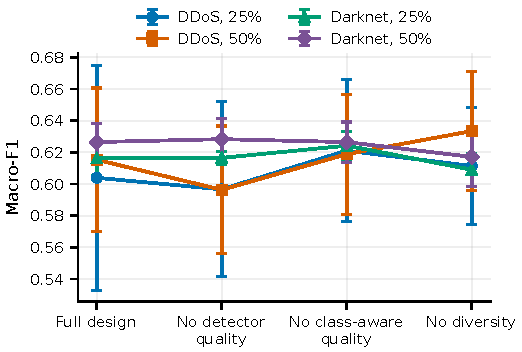
\includegraphics[width=0.96\columnwidth]{figures/eval_component_ablation.pdf}
    \caption{Paired Macro-F1 change after removing one secondary component.
    Points distinguish the 25\% and 50\% budgets; horizontal bars are 95\%
    confidence intervals over five protocol seeds.}
    \label{fig:eval-component-ablation}
\end{figure}

\bheading{Semantic parameters} On two fixed DARKNET partitions and two
architectures, varying $n_{\min}\in\{1,2,5,10\}$ and replacing
inverse-square-root class weights with uniform weights leaves the selected
set, semantic coverage, Macro-F1, and worst recall unchanged across the tested
grid.

\bheading{Learner architecture} We evaluate all four combinations of
XGBoost~\cite{xgboost} and LightGBM local/global
learners.  L+X is best on DDOS, L+L is best on MALDROID and DARKNET, and X+L
and L+L tie on DOH.  The pipeline supports both learner families, with the
strongest backend sensitivity appearing on DDOS.

\begin{table}[t]
    \centering
    \caption{\Fname accuracy for four local/global learner combinations.
    X and L denote XGBoost and LightGBM, respectively; values are means over
    five protocol seeds.}
    \label{tab:eval-architecture}
    \footnotesize
    \setlength{\tabcolsep}{3.8pt}
    \begin{tabular}{@{}lrrrr@{}}
        \toprule
        Dataset & X+X & L+X & X+L & L+L \\
        \midrule
        DDOS     & 0.621 & \textbf{0.642} & 0.641 & 0.624 \\
        MALDROID & 0.826 & 0.854 & 0.847 & \textbf{0.860} \\
        DARKNET  & 0.824 & 0.826 & 0.829 & \textbf{0.832} \\
        DOH      & 0.801 & 0.800 & \textbf{0.807} & \textbf{0.807} \\
        \bottomrule
    \end{tabular}
\end{table}

\bheading{Answer to RQ3} The selected solution is invariant across the tested
semantic-parameter grid, and the pipeline supports all four learner
combinations.  Component and backend choices provide dataset-specific tuning
opportunities.

\subsection{RQ4: What Utility Remains after Laplace Perturbation?}

We can perturb every selected score block before logical upload.  To isolate
utility sensitivity, we freeze the 50\%-budget selection first and
then add independent Laplace noise with scale $2/\epsilon$ to stacker-fit
encodings.  We compare this selected configuration with all 66 encoders on
DDOS over five protocol seeds, keeping test encodings fixed for evaluation.
This centralized replay samples the distribution in
Eq.~\ref{eq:local_laplace_release}; the execution model of
Theorem~\ref{thm:local_score_privacy} instead draws fresh private randomness at
each client before upload.

Table~\ref{tab:eval-laplace} reports Macro-F1 for no noise and
$\epsilon\in\{50,20,10,7,5,3,1\}$.  Here, $\epsilon$ controls the per-block
perturbation and the corresponding noise scale is $2/\epsilon$.  At the
strongest tested perturbation ($\epsilon=1$), Macro-F1 falls from 0.6153 to
0.5105 for the
50\%-budget selection and from 0.6412 to 0.5298 for all encoders.  The
intermediate means fluctuate as $\epsilon$ decreases; the largest observed
drop occurs at $\epsilon=1$.

\begin{table}[t]
    \centering
    \caption{Macro-F1 sensitivity to per-block Laplace perturbation on DDOS.
    Five-seed means are reported with 95\% confidence intervals.}
    \label{tab:eval-laplace}
    \footnotesize
    \setlength{\tabcolsep}{3.0pt}
    \begin{tabular}{@{}lrrr@{}}
        \toprule
        $\epsilon$ & Noise scale & Selected (50\%) & All 66 \\
        \midrule
        No noise & 0     & $0.6153\pm0.0453$ & $0.6412\pm0.0121$ \\
        50       & 0.04  & $0.5861\pm0.0439$ & $0.6037\pm0.0078$ \\
        20       & 0.10  & $0.5932\pm0.0244$ & $0.5999\pm0.0234$ \\
        10       & 0.20  & $0.5910\pm0.0117$ & $0.5918\pm0.0191$ \\
        7        & 0.286 & $0.5939\pm0.0136$ & $0.5874\pm0.0174$ \\
        5        & 0.40  & $0.5875\pm0.0091$ & $0.5777\pm0.0163$ \\
        3        & 0.667 & $0.5655\pm0.0120$ & $0.5870\pm0.0046$ \\
        1        & 2.00  & $0.5105\pm0.0301$ & $0.5298\pm0.0400$ \\
        \bottomrule
    \end{tabular}
\end{table}

\bheading{Answer to RQ4} The seven perturbation levels expose a
utility--perturbation profile: intermediate means fluctuate, while
$\epsilon=1$ produces the largest observed utility drop.  Together with
Theorem~\ref{thm:local_score_privacy}, these results connect the Laplace
release rule to its measured stacker utility.
% TODO(author): The replay does not instantiate a client-side trust boundary.
% End-to-end privacy additionally requires release composition, and the stated
% theorem does not cover labels or the remaining protocol messages.

\subsection{RQ5: Is the Selector and Pipeline Practical?}

\bheading{Exactness and scaling} We first compare the bitmask dynamic program
with exhaustive lexicographic search on a suite of small oracle instances.
The primary coverage value agrees throughout the suite, and repeated runs are
deterministic.  Figure~\ref{fig:eval-solver-scaling} then separates growth in
the number of semantic classes $C$ from growth in the candidate count $M$.
At the main-scale point $M=66,C=12$, the isolated solver uses a median of
1.99 seconds, reaches 2,829 states, and peaks at 98.27 MiB RSS.  Increasing
$M$ to 256 at $C=12$ raises median time to 33.73 seconds, whereas increasing
$C$ to 20 at $M=66$ reaches 460,405 states, 100.10 seconds, and 580.45 MiB.
Thus, semantic dimension, rather than candidate count alone, is the dominant
capacity driver.

\begin{figure}[t]
    \centering
    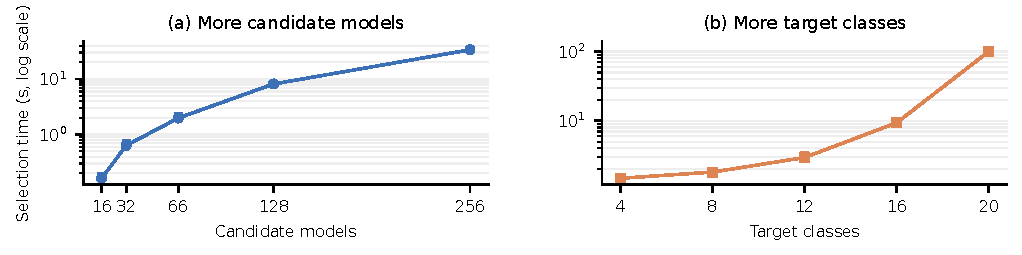
\includegraphics[width=0.96\columnwidth]{figures/eval_solver_scaling.pdf}
    \caption{Sparse dynamic-program scaling.  The blue and rose trajectories
    independently vary semantic classes and candidates using separate fixed
    fixtures.  Both axes are logarithmic; whiskers extend from median to
    95th-percentile time over ten repeats.}
    \label{fig:eval-solver-scaling}
\end{figure}

\bheading{End-to-end replay cost} Table~\ref{tab:eval-system-cost} integrates
wall-clock and logical-communication evidence.  Full
group time includes all reported methods and repetitions, whereas the
preceding microbenchmark isolates one primary solve.  Stacker fitting is the
largest measured stage on MALDROID, DARKNET, and DOH; the multi-method
selection stage is largest on DDOS.  At the 50\% budget, \Fname reduces total
logical payload by approximately half on each dataset.

\begin{table*}[t]
    \centering
    \caption{Single-machine replay time and logical payload.  Times are means
    over five protocol seeds.  ``Dominant'' is the largest recorded stage;
    logical reduction compares \Fname with all encoders.}
    \label{tab:eval-system-cost}
    \footnotesize
    \setlength{\tabcolsep}{3.2pt}
    \begin{tabular}{@{}lrlrrrr@{}}
        \toprule
        Dataset & Total group (s) & Dominant stage & Stage time (s) & All (MiB) & \Fname (MiB) & Reduction \\
        \midrule
        DDOS     & 3,005.16 & Selection     & 1,026.34 & 7,040.05 & 3,489.07 & 50.4\% \\
        MALDROID & 47.03    & Stacker fit   & 35.21    & 662.66   & 335.94   & 49.3\% \\
        DARKNET  & 2,550.50 & Stacker fit   & 2,272.66 & 3,436.78 & 1,732.29 & 49.6\% \\
        DOH      & 512.34   & Stacker fit   & 170.04   & 2,942.76 & 1,488.51 & 49.4\% \\
        \bottomrule
    \end{tabular}
\end{table*}

\bheading{Answer to RQ5} The solver exactly matches exhaustive search
throughout the oracle suite and completes the 66-candidate benchmark in
1.99 seconds.  Scaling isolates semantic dimension as the dominant capacity
driver, while the end-to-end replay confirms an approximately 50\% reduction
in logical payload.
% TODO(author): Exactness is conditioned on completing below the configured
% state cap; physical network latency is outside the current replay.

\endgroup



\section{\red{Discussion}}\label{sec:discuss}

\red{The lexicographic objective answers two distinct deployment questions.
Weighted semantic coverage specifies which source-side class support should
remain whenever the budget permits; the secondary score distinguishes current
prediction behavior only after the best attainable coverage has been fixed.
An instance-specific scalarization can reproduce this order when its minimum
positive coverage gap is known, but no universal finite coefficient works
across arbitrary class weights and candidate pools. The ordered formulation
therefore makes the intended priority explicit. Semantic coverage measures
preserved source-side breadth, while class-conditional Brier lower bounds and
sealed-test metrics measure current competence. The effective-coverage
certificate connects these two views by requiring a selected, source-supported
detector to exceed a deployment-specific class-utility threshold.}

\red{The registered profile sets $\tau_L=1$, so the upper-confidence gate acts
as a finite-sample admissibility screen over normalized Brier risk. The
simultaneous calibration event remains valid after adaptive selection. Within
the resulting pool, the bitmask dynamic program computes the exact primary
value under its registered capacity guard, and the subsequent fill-and-swap
stages preserve that value while providing a one-swap local certificate.}
% TODO(author): A preregistered tau_L<1 experiment would add an
% application-specific population-risk threshold.

\red{Client heterogeneity determines the population described by the
calibration statistics. The implementation targets the record-weighted
client--class mixture. Under stable cell-conditional risks and a deployment
mixture within total variation $\eta$ of the calibration mixture, deployment
Brier risk is at most calibration risk plus $\eta$. The logical-byte budget
then provides a reproducible accounting unit for model delivery and aligned
score blocks across all configurations.}

\red{The privacy protocol asks each client to perturb selected score blocks
with fresh private Laplace randomness before upload. The theorem assigns
$\epsilon_b$ to one block and composes to $s\epsilon_b$ for $s$ selected blocks
of one record. Our centralized sensitivity profile samples the same
post-selection distribution and measures its utility over seven perturbation
levels. A distributed realization places this randomization at each client as
specified by the protocol.}
% TODO(author): The theorem uses public-label, record-level adjacency and a
% cooperative-client threat model.


%Moreover, stronger privacy-enhancing techniques like homomorphic encryption~\cite{acar2018survey} can be implemented together with \Fname to offer stronger privacy protections.

%\tian{Besides the above improvements over \Fname performance, we also plan to incorporate device-dependant feature extractor of raw data into our framework, making it more practical to be deployed. For example, in our experiments, the traffic statistic data are extracted by applying CICFlowMeter~\cite{lashkari2017characterization} on the raw packet data collected using tshark~\cite{merino2013instant}. However, due to the heterogeneity of computational power, the above-mentioned feature extractor may not be the best choice for each device, and a smaller feature extractor, \eg the light-weight feature extractor proposed by Mirsky~\etal~\cite{DBLP:conf/ndss/MirskyDES18} might work better for devices of low computational power.}








\section{Conclusion}
\label{sec:conclusion}
\red{In summary, \Fname integrates pretrained intrusion detectors under a
hard logical-byte budget without changing their parameters. It aligns their
outputs, screens candidates with held-out calibration data, maximizes weighted
semantic coverage exactly under an explicit capacity guard, and refines
current utility and representativeness while preserving that value. Across
four datasets, the 50\% target budget cuts logical payload by 49.3--50.4\% and
closely tracks all-encoder Macro-F1 on MALDROID, DARKNET, and DOH. The selected
detectors feed one shared stacker, and client-side Laplace randomization gives
label-conditional local privacy to uploaded score blocks. Together, the
calibration, solver, privacy, and client-mixture results make post-training
detector integration an auditable deployment decision.}

















% use section* for acknowledgment
% \section*{Acknowledgment}

% Omitted for anonymous review.

% Can use something like this to put references on a page
% by themselves when using endfloat and the captionsoff option.
\ifCLASSOPTIONcaptionsoff
  \newpage
\fi



\bibliographystyle{IEEEtran}
\bibliography{ref} 



% % if you will not have a photo at all:
% \begin{IEEEbiographynophoto}{John Doe}
% Biography text here.
% \end{IEEEbiographynophoto}

% % insert where needed to balance the two columns on the last page with
% % biographies
% %\newpage

% \begin{IEEEbiographynophoto}{Jane Doe}
% Biography text here.
% \end{IEEEbiographynophoto}


\end{document}
